\subsection{Applications}
Because under- and overfill regions affect narrow parts more than wide parts, the use cases for this algorithm are centered around objects which contain thin parts.
Although the algorithm improves performance for all parts compared to existing techniques, the enhancement is percentually larger for thin parts.


\Cref{applications_overview} shows the widths of generated layer toolpaths for various types of 3D model using the inward distributed beading scheme.
Thin parts often occur in architectural models, casings, embossed text, gears and microstructures.
Also in larger regions and organic shapes (\cref{applications_case} and \subref{applications_statue}) our method finds succesful application.

Architectural models and casings benefit from preventing very thin regions from being filled at all and from the prevention of over- and underfill within thin walls, which makes them stronger.
Embossed text benefits from the prevention of underfill areas, which would cause various holes in top surfaces, which is detrimental to the visual quality of those top surfaces.
Gears benefit from the preventio of under- and overfill regions and the distributed bead width discrepancy in that the mechanical properties of the toolpath are more consistent throughout.

Microstructures which have layers with varying widths benefit from the prevention of under- and overfill, which will result in structures with mechanical properties more closely matching homogenized mechanical properties.
For example the result of a topology optimized structure can contain filaments of varying thickness \cite{wu2017infill} which follow a varying stress distribution (\cref{applications_bone}).
Also microstructures with homogenous thickness in the direction perpendicular to the surface of the microstructure can result in horizontal cross-sections with varying thickness;
\cref{applications_gyroid} shows how an angled gyroid structure with homogenous thickness results in heterogeneous outline shapes.
Another class of microstructures consists of homogenous patterns which employ varying thickness in order to achieve a functionally graded material.
\Cref{applications_hex} shows how the toolpathing of a hexagonal grid neatly switches between different bead counts over the volume, which prevents the jagged moves a direction parallel infill pattern would create for such a case. \cite{bates2018compressive}


\begin{figure*}
\centering
\setlength{\figwidth}{0.099\textwidth}
\setlength{\figheight}{0.099\textwidth}
\begin{subfigure}{\textwidth}\centering
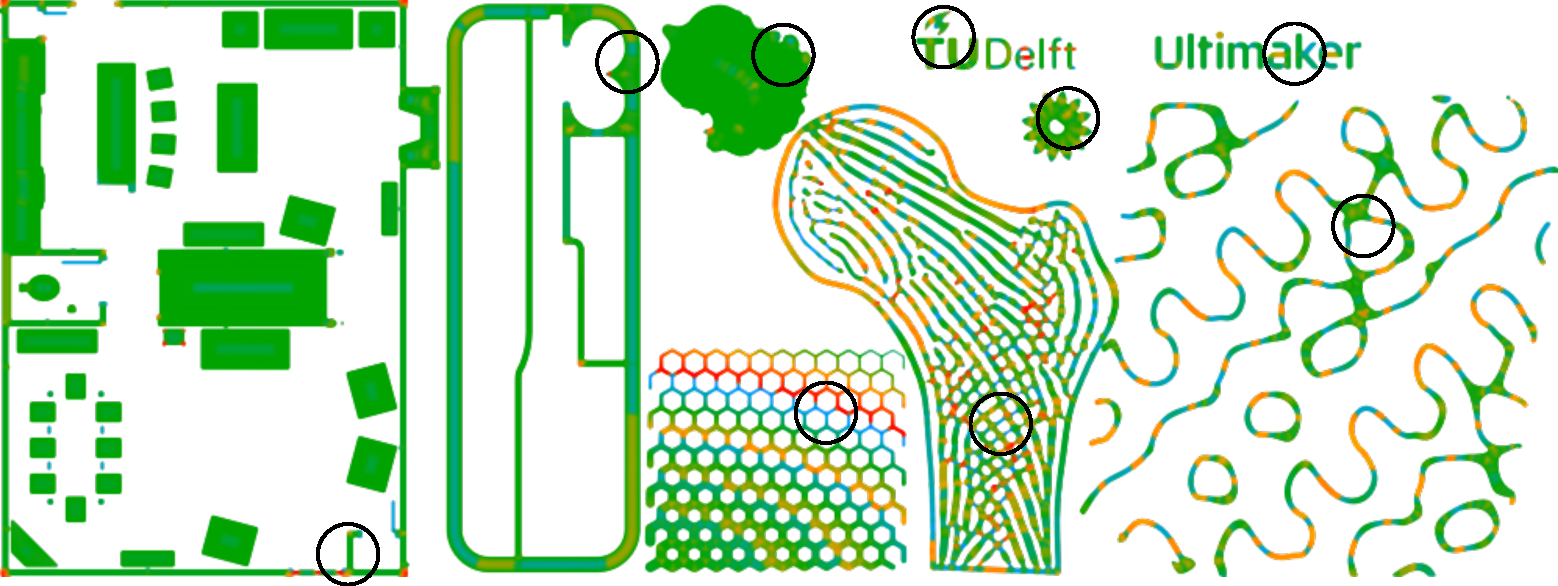
\includegraphics[width=\textwidth]{sources/applications/combined_small_dilated_circled.pdf}
%\caption{Overview}\label{applications_overview}
\end{subfigure}
\begin{subfigure}{\figwidth}\centering
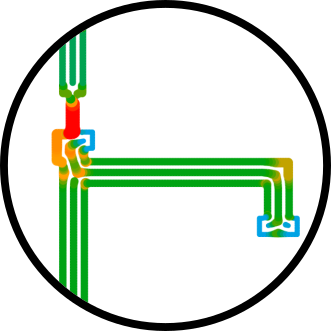
\includegraphics[height=\figheight]{sources/applications/house.png}
\caption{House}\label{applications_house}
\end{subfigure}
\begin{subfigure}{\figwidth}\centering
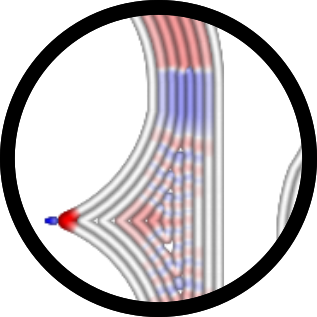
\includegraphics[height=\figheight]{sources/applications/pocket_operator_case.png}
\caption{Case}\label{applications_case}
\end{subfigure}
\begin{subfigure}{\figwidth}\centering
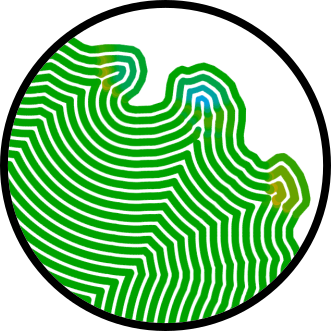
\includegraphics[height=\figheight]{sources/applications/david.png}
\caption{Statue}\label{applications_statue}
\end{subfigure}
\begin{subfigure}{\figwidth}\centering
\censorbox{

\includegraphics[height=\figheight]{sources/applications/tud_logo.png}
}
\caption{\censor{TUD}}\label{applications_tud}
\end{subfigure}
\begin{subfigure}{\figwidth}\centering

\includegraphics[height=\figheight]{sources/applications/ultimaker_logo.png}
\caption{\censor{UM}}\label{applications_um}
\end{subfigure}
\begin{subfigure}{\figwidth}\centering
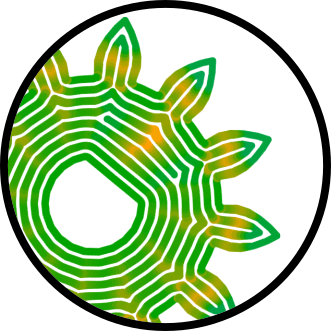
\includegraphics[height=\figheight]{sources/applications/pinion_gear_motor.png}
\caption{Gear}\label{applications_gear}
\end{subfigure}
\begin{subfigure}{\figwidth}\centering
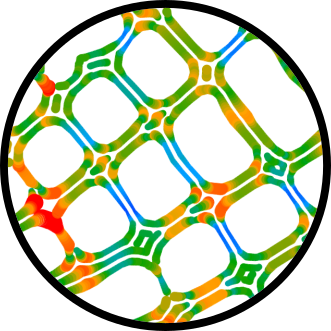
\includegraphics[height=\figheight]{sources/applications/topopt_bone.png}
\caption{Bone}\label{applications_bone}
\end{subfigure}
\begin{subfigure}{\figwidth}\centering
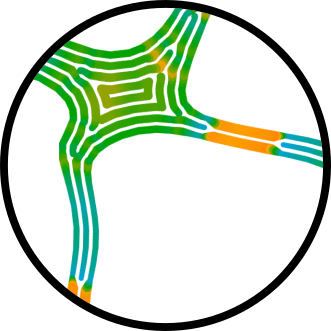
\includegraphics[height=\figheight]{sources/applications/gyroid.png}
\caption{Gyroid}\label{applications_gyroid}
\end{subfigure}
\begin{subfigure}{\figwidth}\centering
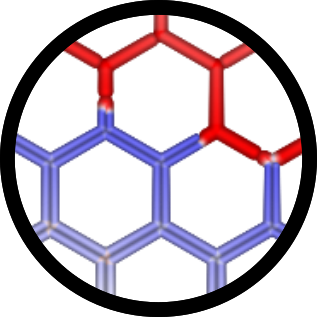
\includegraphics[height=\figheight]{sources/applications/hex_grid.png}
\caption{Hex}\label{applications_hex}
\end{subfigure}
\caption{
Visualization of the widths for the output toolpaths of the inward distributed beading scheme applied to various example application objects.
A legend for the colors can be found in \cref{visualized_accuracy}.
From left to right and top to bottom: a house, a case for electronics, a statue, two logos, a gear, a topologically optimized bone structure, a homogeneous lateral thickness tilted gyroid structure and a heterogeneous thickness hexagonal grid.
}
\label{applications_overview}
\end{figure*}




